%GNUPLOT: LaTeX picture with Postscript
\begin{picture}(0,0)%
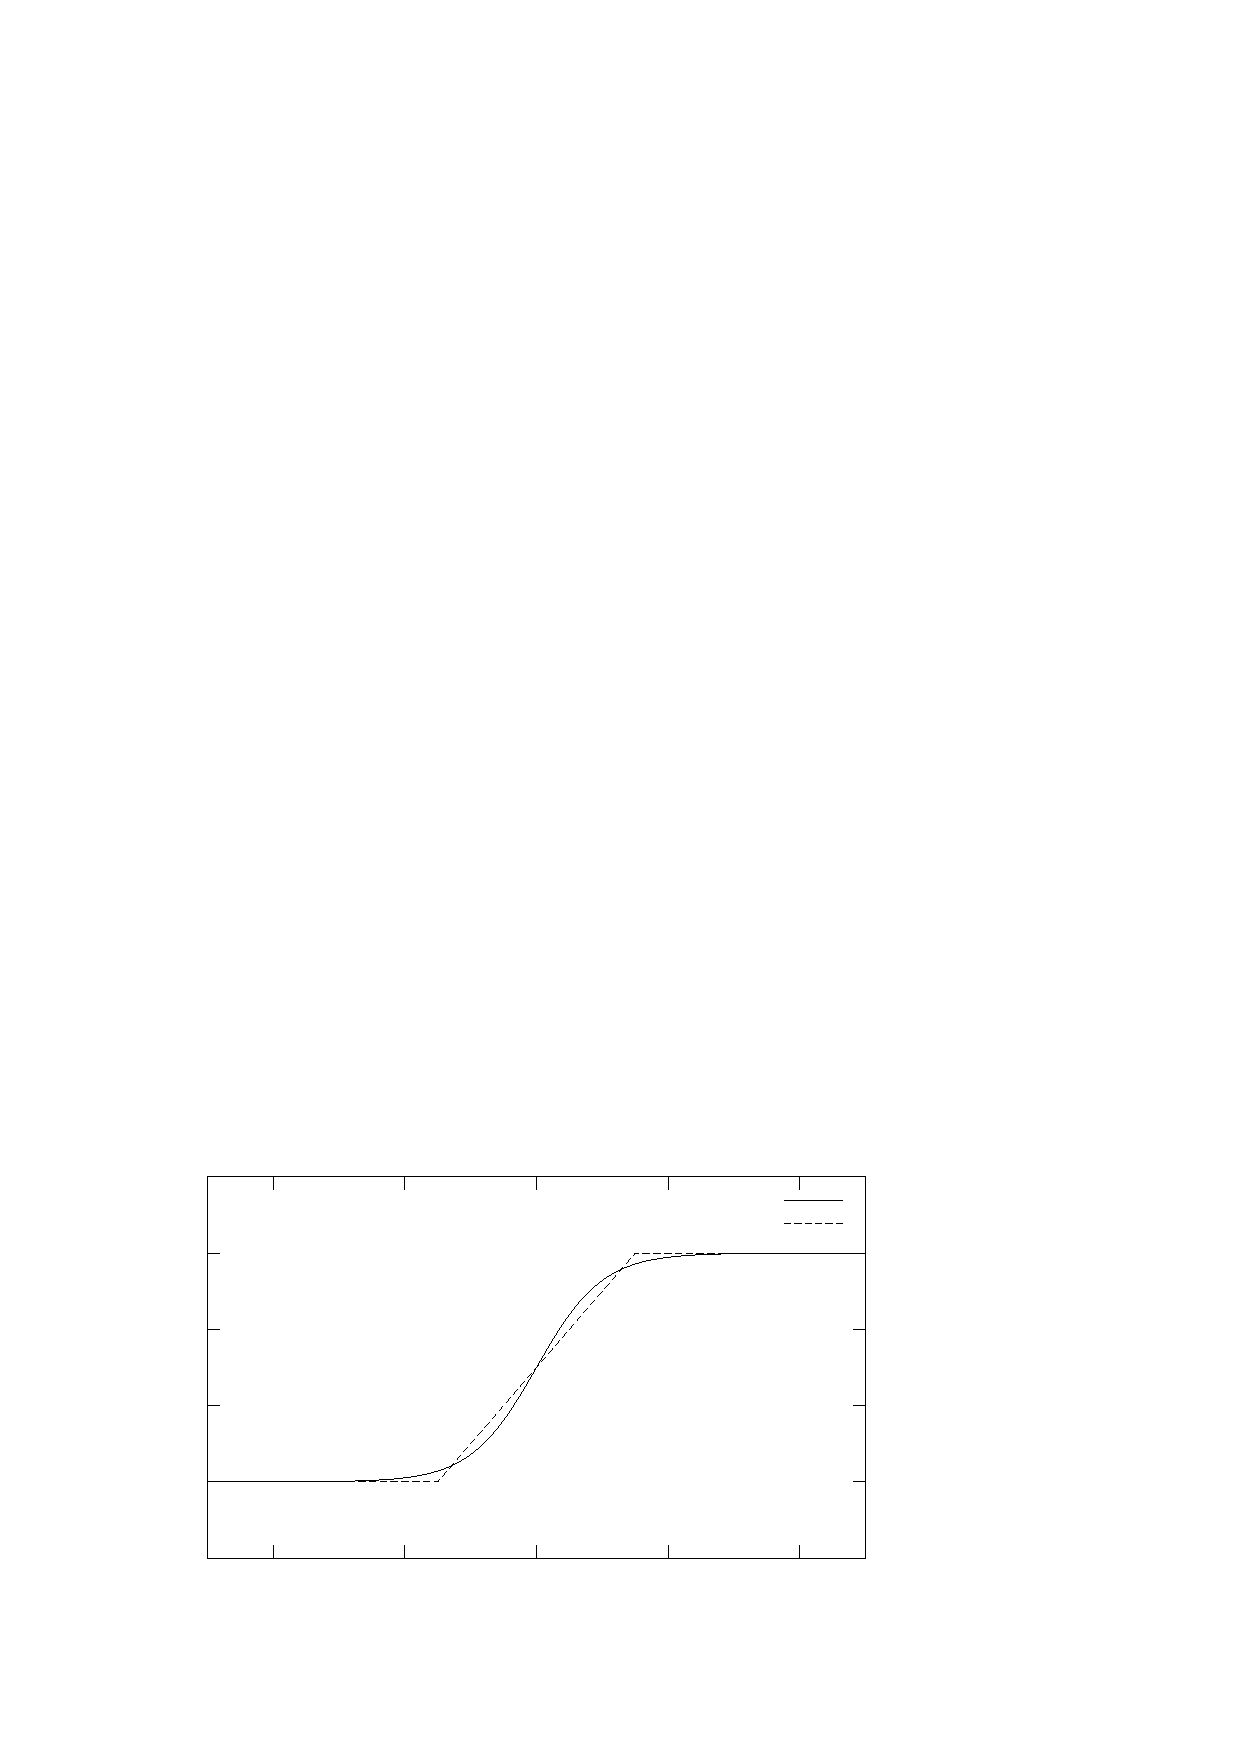
\includegraphics{tanh_pwl}%
\end{picture}%
\begingroup
\setlength{\unitlength}{0.0200bp}%
\begin{picture}(18000,10800)(0,0)%
\put(1100,1100){\makebox(0,0)[r]{\strut{}-1}}%
\put(1100,2930){\makebox(0,0)[r]{\strut{} 0}}%
\put(1100,4760){\makebox(0,0)[r]{\strut{} 1}}%
\put(1100,6590){\makebox(0,0)[r]{\strut{} 2}}%
\put(1100,8420){\makebox(0,0)[r]{\strut{} 3}}%
\put(1100,10250){\makebox(0,0)[r]{\strut{} 4}}%
\put(2955,550){\makebox(0,0){\strut{}-0.4}}%
\put(6115,550){\makebox(0,0){\strut{}-0.2}}%
\put(9275,550){\makebox(0,0){\strut{} 0}}%
\put(12435,550){\makebox(0,0){\strut{} 0.2}}%
\put(15595,550){\makebox(0,0){\strut{} 0.4}}%
\put(14950,9675){\makebox(0,0)[r]{\strut{}ftanh(x)}}%
\put(14950,9125){\makebox(0,0)[r]{\strut{}fpwl(x)}}%
\end{picture}%
\endgroup
\endinput
